\documentclass[12pt]{article}
\usepackage{titling}
\usepackage[absolute]{textpos}
\setlength{\TPHorizModule}{10mm}
\setlength{\TPVertModule}{10mm}
\usepackage[top=2.5cm, bottom=2.5cm, left=3cm, right=2.5cm]{geometry}
\usepackage[polish]{babel}
\usepackage{polski}
\usepackage[utf8]{inputenc}
\usepackage{graphicx}
\usepackage{floatrow}
\usepackage{listings}
\usepackage{color}
\linespread{1.5}
\title{Narzędzie wspomagające tworzenie ciągów przetwarzania wideo w oparciu o bibliotekę GStreamer}
\author{Marcin Kolny}
\usepackage[T1]{fontenc}
\usepackage{helvet}
\renewcommand*{\familydefault}{\sfdefault}
\renewcommand{\maketitle}{
  \begin{titlepage}
    \begin{figure}  
      
\includegraphics[width=40mm]{img/polsl-logo.png}
    \end{figure}
    \begin{center}
      \begingroup
      \fontsize{18pt}{21pt}\selectfont
      \textbf{Politechnika Śląska\\
        Wydział Automatyki, Elektroniki i Informatyki\\
        Kierunek Informatyka}\\
      \vspace{22mm}
      Projekt inżynierski\\
      \vspace{22mm}
      \endgroup
      \begingroup
      \fontsize{14pt}{17pt}\selectfont
      \thetitle \\
      \endgroup
      \vspace{30mm}
    \end{center}
    \begin{textblock}{14}(2.5,21.5)
      \fontsize{14pt}{17pt}\selectfont
      Autor: \theauthor \\
      Kierujący pracą: dr Ewa Lach\\
    \end{textblock}
    \begin{textblock}{20}(2.5,26.5)
      \fontsize{14pt}{17pt}\selectfont
      Gliwice, styczeń 2014\\
    \end{textblock}

  \end{titlepage}
}
\begin{document}
\definecolor{cppred}{rgb}{0.6,0,0} % strings
\definecolor{cppgreen}{rgb}{0.25,0.5,0.35} % comments
\definecolor{cpppurple}{rgb}{0.5,0,0.35} % keywords
\definecolor{cppblue}{rgb}{0.25,0.35,0.75} % doxygen
\definecolor{lightgrey}{rgb}{0.9,0.9,0.9}
\lstset{language=C++,
basicstyle=\ttfamily,
keywordstyle=\color{cpppurple}\bfseries,
stringstyle=\color{cppred},
commentstyle=\color{cppgreen},
morecomment=[s][\color{cppblue}]{/**}{*/},
numbers=left,
backgroundcolor=\color{lightgrey},
numberstyle=\tiny\color{black},
stepnumber=1,
numbersep=10pt,
tabsize=4,
showspaces=false,
showstringspaces=false}
\maketitle
\tableofcontents
\cleardoublepage
\textbf{\Large Założenia projektowe} \\
Celem projektu jest stworzenie oprogramowania, umożliwiającego w łatwy i wygodny sposób projektować programy przetwarzające strumienie multimedialne, w oparciu o bibliotekę GStreamer. Funkcjonalność programu zawiera się w niżej wymienionych punktach.
\begin{itemize}
 \setlength{\itemsep}{0em}
\item Tworzenie programu metodą \textit{przeciągnij-upuść} (ang. \textit{drag\&drop}). Dzięki temu, nawet osoba nie posiadająca wiedzy na temat tworzenia oprogramowania, będzie mogła stworzyć własny program.
\item Zapis projektu do pliku i powtórne załadowanie projektu do programu. Założeniem jest, że użytkownik będzie chciał w przyszłości zmodyfikować wcześniej utworzony program. Zapisywanie i odczytywanie plików projektu umożliwi osobom korzystającym z programu późniejsze modyfikacje swojego projektu.
\item Generowanie kodu źródłowego na podstawie projektu. Aplikacja powinna nie tylko dawać możliwość prototypowania programu. Prototyp może rozrosnąć się do bardzo dużych rozmiarów, co później może powodować problemy w implementacji. Automatyczne generowanie kodu na podstawie utworzonego prototypu zwolni użytkownika z obowiązku żmudnej pracy przepisywania kodu źródłowego.
\item Wyświetlanie wiadomości pochodzących z biblioteki GStreamer. Biblioteka GStreamer wysyła użytkownikowi wiele komunikatów informujących o przebiegu wykonania programu. Użytkownik powinien mieć możliwość śledzenia, a także filtrowania tych informacji, w celu poprawienia błędów w swojej aplikacji.
\end{itemize}
\cleardoublepage
\section{Analiza problemu}
\subsection{Narzędzia}
\subsubsection{Biblioteka GStreamer}
\paragraph{}
Biblioteka GStreamer służy do konstruowania grafów przetwarzania strumieni multimedialnych. Biblioteka została napisana w języku ANSI C i dostępna jest pod systemami Linux, Windows, OS X oraz Android.

GStreamer wydany jest na licencji GNU GPL i może być wykorzystywany w zastosowaniach komercyjnych. Licencja pozwala również na modyfikowanie i dystrybucję kodu źródłowego biblioteki.
Biblioteka oferuje użytkownikowi wiele gotowych elementów do przetwarzania wideo (np. enkodery czy dekodery audio-video), do generowania sygnałów multimedialnych, a także do prezentacji wyników użytkownikowi. Ponadto, istnieje możliwość pisania własnych elementów, które można następnie użyć w bilbliotece GStreamer.

Biblioteka GStreamer oparta jest o \textbf{elementy} (ang. \textit{elements}). Elementem nazywany jest obiekt, który realizuje zadany algorytm. Przykładowym elementem jest dekoder, którego celem jest dekodowanie strumienia multimedialnego o zadanym formacie.

Element może zawierać gniazda, dzięki którym możliwe jest połączenie go z innymi elementami.

Elementy dzielą się na te, które zawierają tylko gniazda wejściowe (ang. \textit{sink elements}), które posiadają tylko gniazda wejściowe (ang. \textit{source elements}), oraz elementy zawierające zarówno gniazda wejściowe, jak i wyjściowe (ang. \textit{filter elements}).
\begin{figure}[H]
  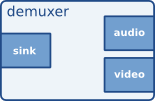
\includegraphics[width=40mm]{img/sample-demuxer.png}
  \caption{Przykładowy element typu \textit{demuxer} \cite{gstmainpage}}
  \label{fig:sampleDemuxer}
\end{figure}
\paragraph{}
Rysunek ~\ref{fig:sampleDemuxer} przedstawia przykładowy element, zawierający dwa gniazda wyjściowe, i jedno gniazdo wejściowe (jest to szczególny wariant filtra, tzw. \textit{demuxer}).
\paragraph{}
\textbf{Kontener} (ang. \textit{bin}) jest szczególnym elementem. Podobnie, jak elementy, kontenery posiadają gniazda. Natomiast algorytmy zdefiniowane w elemencie-kontenerze realizowane są poprzez inne elementy, które agregowane są w danym kontenerze. Rysunek ~\ref{fig:sampleBin} przedstawia przykładowy kontener, zawierający dwa elementy, oraz jedno gniazdo wejściowe.
\begin{figure}[H]
  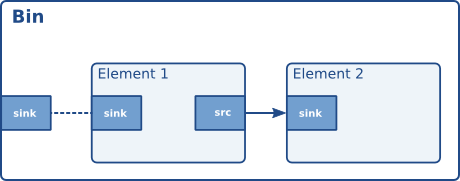
\includegraphics[width=100mm]{img/sample-bin.png}
  \caption{Przykładowy kontener \cite{gstmainpage}}
  \label{fig:sampleBin}
\end{figure}
\paragraph{}
\textbf{Strumień} (ang. \textit{pipeline}) jest specjalnym przypadkiem kontenera. Jest to kontener nadrzędny całego modelu programu. Przechowuje w sobie główne elementy oraz kontenery agregujące inne obiekty przetwarzające. Strumień nie posiada żadnych gniazd. Rysunek ~\ref{fig:samplePipeline} przedstawia przykładowy strumień, realizujący operację odtwarzania strumienia audio-video z pliku ogg.
\begin{figure}[H]
  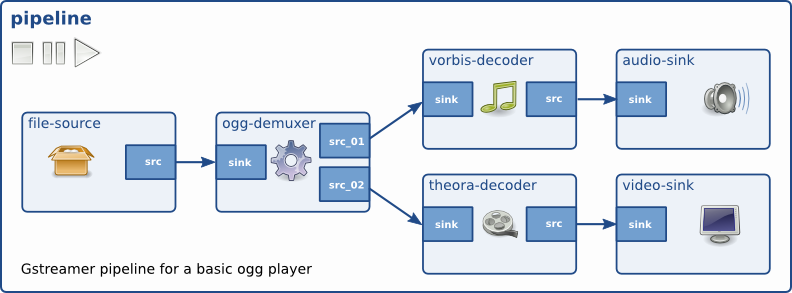
\includegraphics[width=150mm]{img/simple-player.png}
  \caption{Przykładowy strumień \cite{gstmainpage}}
  \label{fig:samplePipeline}
\end{figure}
\paragraph{}
\textbf{Gniazda} (ang. \textit{pads}) to obiekty umożliwiające połączenie ze sobą dwóch różnych elementów. Gniazdo charakteryzuje się dwoma właściwościami: kierunkiem oraz dostępnością. Pod względem kierunku, gniazda podzielone są na dwie grupy:
\begin{itemize}
 \setlength{\itemsep}{0em}
  \item wejściowe (ang. \textit{sink pads}),
  \item wyjściowe (ang. \textit{src pads}).
\end{itemize}

Gniazda wyjściowe (źródłowe), służą do przesyłania danych do następnego elementu. Gniazda wejściowe wykorzystywane są natomiast do odbierania danych przesłanych z poprzednich elementów.

Kolejna właściwość, dzieli zbiór gniazd na trzy grupy:
\begin{itemize}
 \setlength{\itemsep}{0em}
  \item występujące zawsze (ang. \textit{always pads}),
  \item występujące w zależności od danych (ang. \textit{sometimes pads, dynamic pads}),
  \item pojawiające się na żądanie użytkownika (ang. \textit{request pads}).
\end{itemize}

Gniazda należące do pierwszej grupy występują zawsze w elemencie, i nie można ich usunąć.
Druga grupa gniazd, to takie, które pojawiają się tylko wtedy, kiedy wystąpi taka potrzeba. Na rysunku ~\ref{fig:requestPadsDemux} pokazane zostały dwa demultiplexery połączone z elementem wczytującym dane z pliku. W pierwszym przypadku (po lewej), w pliku zapisane zostały dwa strumienie multimedialne, dlatego element \textit{ogg-demuxer} zawiera dwa gniazda źródłowe. W drugim przypadku (po lewej), plik zawiera tylko jeden strumień multimedialny, stąd demuxer wygenerował tylko jedno gniazdo.
\begin{figure}[H]
  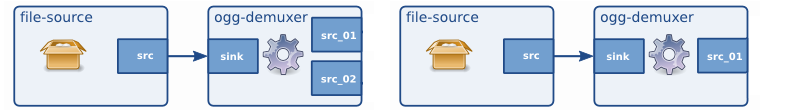
\includegraphics[width=150mm]{img/request-pads-demux.png}
  \caption{Dynamiczne gniazda elementu demuxera \cite{gstmainpage}}
  \label{fig:requestPadsDemux}
\end{figure}
Ostatnia grupa, to gniazda, pojawiające się na żądanie użytkownika. Można wyobrazić sobie odwrotną sytuację do opisywanej w poprzednim akapicie. Użytkownik wstawia element typu \textit{muxer}, który łączy kilka strumieni. W zależności od tego, ile strumieni użytkownik będzie chciał połączyć, tyle żądań o gniazdo wejściowe będzie musiał zgłosić.

\textbf{Połączenia} (ang. \textit{links}) pomiędzy dwoma elementami odbywają się przez tzw. \textit{negocjacje}. Każde gniazdo elementu posiada właściwość określającą, jakiego typu dane akceptuje dane gniazdo. Właściwości te nazywane są możliwościami (ang. \textit{capabilities}, \textit{caps}). Proces negocjacji ma na celu odnalezienie wspólnego formatu danych, jaki może zostać zaakceptowany przez odybwa gniazda (gniazdo wejściowe oraz wyjściowe), które użytkownik chce ze sobą połączyć. Jeśli negocjacje zakończą się niepowodzeniem (to znaczy, nie uda się znaleźć wspólnego formatu), połączenie nie zostanie wykonane.

\subsubsection{Adapter C++ - gstreamermm}
\paragraph{}
Adapter (ang. \textit{wrapper}) jest wzorcem projektowym, który ma na celu współdzielenie interfejsu pomiędzy dwoma blokami kodu źródłowego. Biblioteka GStreamer została napisana w języku ANSI C, dlatego, aby umożliwić programistom innych języków korzystanie z biblioteki, nie mieszając różnych języków, powstało kilka adapterów dla innych języków programowania (np. C++ czy C\#).

Biblioteka \textbf{gstreamermm} to projekt, którego celem jest stworzenie biblioteki-adaptera w języku C++ dla biblioteki GStreamer. Projekt rozwijany jest na licencji LGPL, dlatego każdy może uzyskać dostęp do kodu źródłowego biblioteki, a także w dowolny sposób modyfikować źródła.

Biblioteka gstreamermm należy do rodziny projektów pochodzących od projektu biblioteki-wrappera \textbf{gtkmm}. Biblioteka gtkmm umożliwia użytkownikowi korzystanie z funkcjonalności biblioteki GTK+, posługując się interfejsem napisanym w języku C++. Projekty oparte o fragmenty kodu biblioteki gtkmm, opierają się głównie o generowanie kodu źródłowego w języku C++ na podstawie źródeł napisanych w języku ANSI C. Wszystkie projekty korzystają ze wspólnych generatorów kodu, dlatego każde usprawnienie generatora w jednym projekcie, powoduje polepszenie jakości kodu w pozostałych projektach..

Kod źródłowy biblioteki jest w większości generowany automatycznie na podstawie źródeł projektu GStreamer w trójetapowym procesie. Rysunek ~\ref{fig:mmGenerateProcess} prezentuje wszystkie trzy kroki procesu generacji kodu źródłowego.
\begin{figure}[H]
  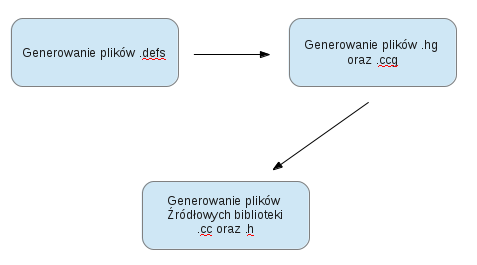
\includegraphics[width=100mm]{img/mm-generate-process.png}
  \caption{Schemat procesu generacji kodu źródłowego biblioteki gstreamermm}
  \label{fig:mmGenerateProcess}
\end{figure}
Pierwszym etapem generacji kodu jest przeszukanie źródeł biblioteki GStreamer, a następnie wygenerowanie plików definicji. Pliki definicji zawierają informacje na temat typów wyliczeniowych zdefiniowanych w bibliotece, funkcji, sygnałów, metod wirtualnych czy struktur danych. W przypadku wygenerowania przez generator błędnej definicji, stosowane są pisane przez programistę tzw. \textit{łatki} (ang. \textit{patch}).

W kolejnym przebiegu, generator na podstawie plików definicji, generuje pliki \textit{.hg} oraz \textit{.ccg}. Zawartość plików przypomina składnią język C++, jednak zawiera wywołania makrodefinicji ułatwiających adaptowanie poszczególnych elementów biblioteki. Przykład użycia makrodefinicji przedstawiony został na listingu ~\ref{macroSampleUsage}.
Listę dostępnych makr można znaleźć w dokumentacji projektu gnome \cite{devgnomepage}.
    \begin{lstlisting}[caption=Przykład użycia makrodefinicji w pliku \textit{.hg}, label=macroSampleUsage]
_WRAP_METHOD(bool load_preset(const Glib::ustring& name), 
      gst_preset_load_preset)
    \end{lstlisting}
    W przypadku, gdy plik \textit{.hg} zostanie niepoprawnie wygenerowany, programista zmuszony jest do ręcznego napisania tego pliku. W tym wypadku nie stosuje się łatek, ponieważ w większości przypadków, błąd obejmuje większą część pliku, a nie pojedyncze linie.

Ostatni etap generacji kodu źródłowego, to przekształcenie plików \textit{.hg} oraz \textit{.ccg} w pliki źródłowe języka C++. Na przykład, line pokazane na listingu ~\ref{macroSampleUsage} zostanie zastąpione kodem zaprezentowanym na listingu ~\ref{outMacroSampleUsage}.
    \begin{lstlisting}[caption=Kod źródłowy wygenerowany na podstawie makrodefinicji, label=outMacroSampleUsage]
bool load_preset(const Glib::ustring& name);
...
bool Preset::load_preset(const Glib::ustring& name)
{
  return gst_preset_load_preset(gobj(), name.c_str());
}
    \end{lstlisting}
    Funkcja \textit{gst\_preset\_load\_preset} jako drugi argument, przyjmuje wartość typu \textit{gchar*}. Generator wiedział, w jaki sposób dokonać konwersji na ten typ z typu \textit{const Glib::ustring\&}. Baza wiedzy, dotycząca konwersji pomiędzy typami ANSI C a typami języka C++, znajduje się w osobnych plikach, pisanych przez programistę.
W tym etapie, wygenerowany kod źródłowy jest zawsze poprawny. Programista może jedynie dopisać dodatkowe pliki. Przechowują one na ogół klasy usprawniające (ale nie rozszerzające funkcjonalność) pracę z biblioteką.
\cleardoublepage
\section{Specyfikacja zewnętrzna}
Program powinien być uruchamiany pod systemem operacyjnym Linux. Wymaga on zainstalowanej biblioteki gstreamermm 1.0.
\subsection{Proces instalacji biblioteki gstreamermm}
Na listingu ~\ref{gstreamermmInstall} przedstawiona została lista poleceń, jakie należy wykonać w celu instalacji biblioteki gstreamermm. Proces instalacji wymaga połączenia z internetem, ponieważ źródła biblioteki muszą zostać pobrane ze zdalnego repozytorium.
\begin{lstlisting}[caption=Polecenia kompilujące program gst-creator, label=gstreamermmInstall]
[m.kolny@m.kolny-cmp ~]$ git clone git://
                             git.gnome.org/gstreamermm
[m.kolny@m.kolny-cmp ~]$ cd gstreamermm
[m.kolny@m.kolny-cmp gstreamermm]$ 
[m.kolny@m.kolny-cmp gstreamermm]$ ./autogen.sh
[m.kolny@m.kolny-cmp gstreamermm]$ make
[m.kolny@m.kolny-cmp gstreamermm]$ sudo make install
\end{lstlisting}

\textbf{Wymagane zależności dla kompilacji biblioteki}\\
Poniżej znajduje się lista zależności, jakie muszą zostać spełnione w celu poprawnej kompilacji i instalacji biblioteki gstreamermm:
\begin{itemize}
  \setlength{\itemsep}{0em}
\item narzędzie mm-common w wersji 0.9.6 lub wyższej,
\item biblioteka giomm-2.4 w wersji 2.36.0 lub wyższej,
\item biblioteka gstreamer-1.0 w wersji 1.0.10 lub wyższej,
\item biblioteka gstreamer-app-1.0 w wersji 1.0.10 lub wyższej,
\item biblioteka gstreamer-audio-1.0 w wersji 1.0.10 lub wyższej,
\item biblioteka gstreamer-base-1.0 w wersji 1.0.10 lub wyższej,
\item biblioteka gstreamer-check-1.0 w wersji 1.0.10 lub wyższej,
\item biblioteka gstreamer-controller-1.0 w wersji 1.0.10 lub wyższej,
\item biblioteka gstreamer-fft-1.0 w wersji 1.0.10 lub wyższej,
\item biblioteka gstreamer-net-1.0 w wersji 1.0.10 lub wyższej,
\item biblioteka gstreamer-pbutils-1.0 w wersji 1.0.10 lub wyższej,
\item biblioteka gstreamer-plugins-base-1.0 w wersji 1.0.10 lub wyższej,
\item biblioteka gstreamer-riff-1.0 w wersji 1.0.10 lub wyższej,
\item biblioteka gstreamer-rtp-1.0 w wersji 1.0.10 lub wyższej,
\item biblioteka gstreamer-sdp-1.0 w wersji 1.0.10 lub wyższej,
\item biblioteka gstreamer-tag-1.0 w wersji 1.0.10 lub wyższej,
\item biblioteka gstreamer-video-1.0 w wersji 1.0.10 lub wyższej.
\end{itemize}
Ponadto, w celu kompilacji przykładowych programów wykorzystujących bibliotekę gstreamermm, w systemie musi być zainstalowana biblioteka gtkmm-3.0 w wersji 3.0 lub wyższej.
\subsection{Proces instalacji programu}
Oprogramowanie dostarczane jest w postaci kodu źródłowego, dlatego w celu uruchomienia programu, należy dokonać kompilacji programu. Skrypt budujący został przygotowany pod narzędzie \textbf{CMake}. Aby skompilować program, należy wykonać polecenia w konsoli przedstawione na listingu ~\ref{compileProject} (użytkownik powinien znajdować się w katalogu głównym repozytorium programu).
\begin{lstlisting}[caption=Polecenia kompilujące program gst-creator, label=compileProject]
[m.kolny@m.kolny-cmp gst-creator]$ mkdir build
[m.kolny@m.kolny-cmp gst-creator]$ cd build/
[m.kolny@m.kolny-cmp build]$ cmake ..
[m.kolny@m.kolny-cmp build]$ make
\end{lstlisting}
Polecenia spowodują skompilowanie aplikacji w katalogu build. Skompilowany plik wykonywalny znajduje się w katalogu \textbf{./build/src/} pod nazwą \textbf{gst-creator}. \\
\textbf{Zależności kompilacji programu} \\
Kompilacja programu gst-creator wymaga spełnienia następujących zależności:
\begin{itemize}
  \setlength{\itemsep}{0em}
\item CMake w wersji 2.8.9 lub wyższej,
\item gstreamermm w wersji 1.0
\item GTest w wersji 1.6 lub wyższej.
\end{itemize}
\subsection{Automatyczna kompilacja i instalacja zależności oraz aplikacji}
W celu uproszczenia procesu kompilacji aplikacji, przygotowałem skrypt, mający na celu automatyczne rozwiązywanie zależności. Skrypt został przetestowany na świeżej instalacji systemu operacyjnego Ubuntu 13.04 i386. Aby uruchomić skrypt automatycznej instalacji, należy wykonać polecenia pokazane na listingu ~\ref{autoinstallerRunner}.
\begin{lstlisting}[caption=Uruchomienie skryptu autoinstalatora, label=autoinstallerRunner]
[m.kolny@m.kolny-cmp gst-creator]$ chmod +x bootstrap.sh
[m.kolny@m.kolny-cmp gst-creator]$ ./bootstrap.sh
\end{lstlisting}
\subsection{Instrukcja obsługi}
\subsubsection{Uruchomienie programu}
Aby uruchomić program, należy wykonać polecenie przedstawione na listingu ~\ref{runApp}. Uruchomienie programu nie wymaga żadnych dodatkowych plików.
\begin{lstlisting}[caption=Uruchomienie programu, label=runApp]
[m.kolny@m.kolny-cmp build]$ ./src/gst-creator $
\end{lstlisting} 
\subsubsection{Główne okno programu}
Po uruchomieniu aplikacji użytkownikowi ukaże się główne okno programu. Składa się ono z ośmiu podstawowych modułów, które zostały oznaczone na rysunku ~\ref{fig:mainWindow}. Poniżej w skrócie zostaną omówione poszczególne elementy głównego okna programu.
\begin{figure}[H]
  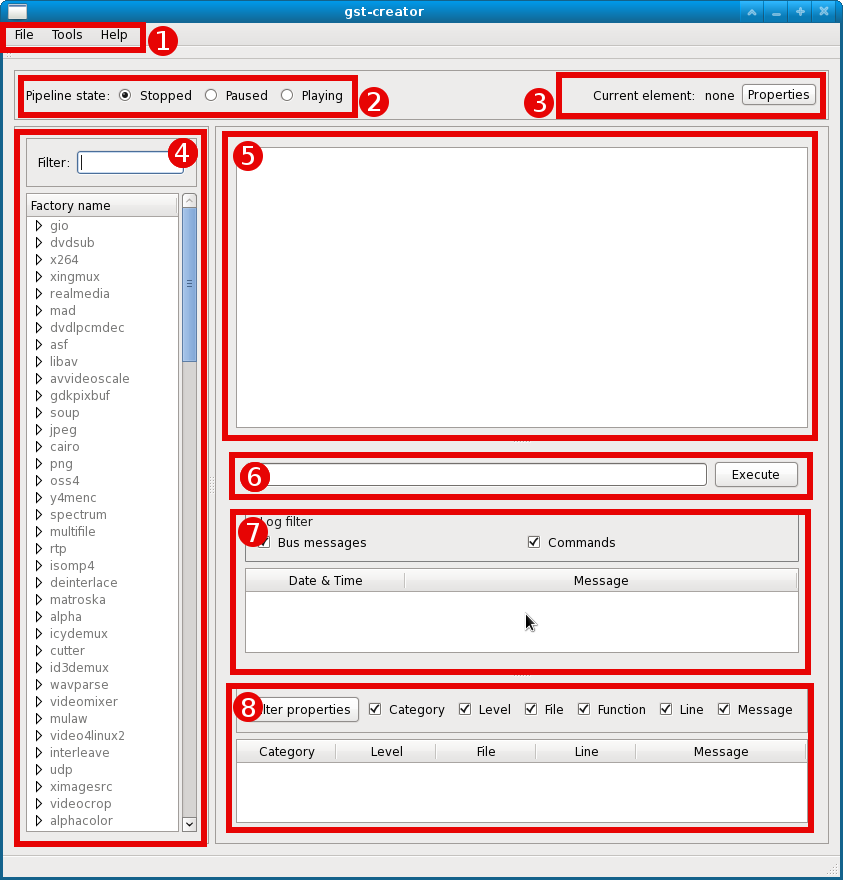
\includegraphics[width=160mm]{img/main-window.png}
  \caption{Zrzut ekranu głównego okna programu}
  \label{fig:mainWindow}
\end{figure}
\begin{enumerate}
  \setlength{\itemsep}{0em}
\item Główne menu programu - umożliwia dostęp do podstawowych operacji związanych z plikiem projektu. Ponadto daje użytkownikowi możliwość skorzystania z dodatkowych narzędzi takich jak generator kodu źródłowego czy kreator wtyczek.
\item Wskaźnik stanu modelu programu - pozwala użytownikowi śledzić oraz zmieniać aktualny stan, w jakim znajduje się model programu.
\item Aktualnie zaznaczony element - informuje użytkownika o tym, jaki element jest w danej chwili zaznaczony. Daje również możliwość do szybkiej zmiany właściwości zaznaczonego elementu.
\item Inspektor elementów - zawiera listę wszystkich dostępnych elementów, jakie mogą zostać wykorzystane przez użytkownika przy tworzeniu modelu programu.
\item Obszar roboczy programu - miejsce, w którym użytkownik składa z dostępnych elementów reprezentowanych przez bloczki model programu.
\item Wiersz poleceń - umożliwia tworzenie modelu programu poprzez wydawanie odpowiednich poleceń do programu.
\item Konsola logowania zdarzeń programu - przechwytuje i wyświetla zdarzenia pochodzące z aplikacji oraz z magistrali.
\item Konsola logowania zdarzeń GStreamera - przechwytuje i wyświetla zdarzenia pochodzące z biblioteki GStreamer.
\end{enumerate}\paragraph{}\vspace{-3mm}
\textbf{Główne menu programu} \\
Główne menu programu umożliwia użytkownikowi dostęp do następujących funkcjonalności:
\begin{itemize}
  \setlength{\itemsep}{0em}
\item utworzenie nowego projektu (\textit{File->New Project...}),
\item załadowanie istniejącego projektu (\textit{File->Open Project...}),
\item zapis aktualnie edytowanego projektu (\textit{File->Save}, \textit{File->Save As...}),
\item załadowanie istniejącej wtyczki do inspektora obiektu (\textit{File->Load Plugin...}),
\item dodanie ścieżki przeszukiwania wtyczek przez inspektora obiektu (\textit{File->Add Plugin Path...}),
\item zamknięcie programu (\textit{File->Exit}),
\item wywołanie narzędzia kreatora wtyczki (\textit{Tools->Plugin Wizzard...}),
\item wywołanie narzędzia generatora kodu (\textit{Tools->Code Generator...}),
\item wyświetlenie informacji o programie (\textit{Help->About GstCreator}).
\end{itemize}
\paragraph{}\vspace{-3mm}
\textbf{Wskaźnik stanu modelu programu} \\
Model programu może przyjmować trzy stany:
\begin{itemize}
\item stan zatrzymania (\textit{Stopped}),
\item stan pauzy (\textit{Paused}),
\item stan odtwarzania (\textit{Playing}).
\end{itemize}
Wskaźnik stanu modelu pozwala nie tylko na podejrzenie aktualnego stanu modelu, ale również na jego zmianę. \paragraph{}\vspace{-3mm}
\textbf{Aktualnie zaznaczony element} \\
Moduł aktualnie zaznaczonego elementu ma na celu przedstawić użytkownikowi element, który jest aktualnie zaznaczony. Ponadto, użytkownik ma możliwość szybkiego dostępu do własciwości elementu. Po wciśnięciu przycisku \textit{Properties}, zostanie wyświetlone kolejne okienko programu (rysunek ~\ref{fig:allPropertiesWindow}). \paragraph{}\vspace{-3mm}
\textbf{Inspektor elementów} \\
Inspektor elementów daje możliwość przejrzenia wszystkich dostępnych wtyczek (ang. \textit{plug-ins}) biblioteki GStreamer. Pozwala również na wyświetlenie informacji na temat zawartych w nich fabryk elementów, wraz ze szczegółowymi danymi każdej fabryki elementów. 
Lista wtyczek oraz dostępnych w nich fabryk wizualizowana jest w postaci drzewa obiektów. Wtyczka jest elementem nadrzędnym dla fabryki elementów. Oprócz tego moduł zawiera wyszukiwarkę, która umożliwia przeszukiwanie listy obiektów (rysunek ~\ref{fig:elementInspector}).
W celu uzyskania informacji na temat konkretnej wtyczki, należy skierować kursor na nazwę danej wtyczki, a następnie dwukrotnie kliknąć na wskazany obiekt. Na ekranie użytkownika pokaże się okno (rysunek ~\ref{fig:matroskaInspectWindow}), zawierające informację na temat wtyczki:
\begin{itemize}
  \setlength{\itemsep}{0em}
\item nazwa,
\item opis,
\item ścieżka do pliku,
\item wersja,
\item licencja,
\item moduł źródłowy,
\item data wydania,
\item pakiet, w skład którego wchodzi wtyczka,
\item pochodzenie pakietu.
\end{itemize}
\begin{figure}[H]
  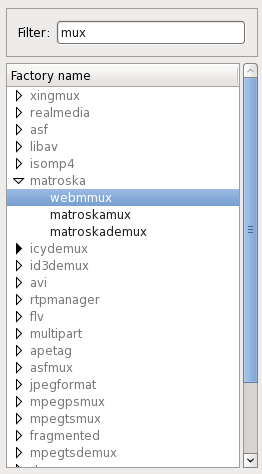
\includegraphics[width=7cm]{img/element-inspector.png}
  \caption{Wyszukiwanie frazy w inspektorze elementów}
  \label{fig:elementInspector}
\end{figure}
\noindent
Aby uzyskać dostęp do informacji na temat konkretnej fabryki elementów, należy dwukrotnie kliknąć na obiekt inspektora elementów reprezentujący daną fabrykę. Spowoduje to wyświetlenie okna właściwości fabryki (rysunek ~\ref{fig:xingmuxFactoryInfoWindow}). Informacje rozmieszczone są w oknie w pięciu grupach.
\begin{figure}[H]
  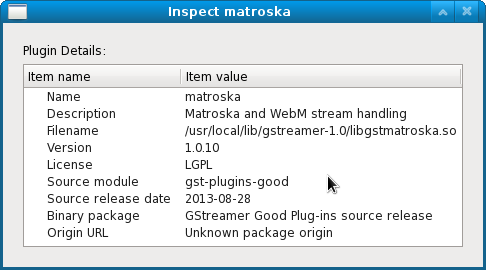
\includegraphics[width=12cm]{img/matroska-inspect-window.png}
  \caption{Okno właściwości wtyczki \textit{matroska}}
  \label{fig:matroskaInspectWindow}
\end{figure}
\begin{itemize}
  \setlength{\itemsep}{0em}
\item Szczegóły fabryki (ang. \textit{factory details}) - wyświetla podstawowe informacje na temat fabryki:
  \begin{itemize}
    \setlength{\itemsep}{0em}
  \item \textit{długą nazwę} fabryki,
  \item klasę, do jakiej przynależy fabryka,
  \item opis,
  \item autora.
  \end{itemize}
\item Szablony gniazd (ang. \textit{pad templates}) - wyświetla wszystkie dostępne szablony gniazd, a także informacje o kompatybilnych formatach multimedialnych. Formaty wyświetlane są w postaci drzewa, tak, aby użytkownik mógł w łatwy sposób wyszukać pożądany format.
\item Gniazda (ang. \textit{pads}) - agreguje informacje na temat statycznych gniazd.
\item Właściwości (ang. \textit{properties}) - prezentuje informacje dotyczące właściwości zdefiniowanych w danej fabryce elementów. Wyświetla informacje dotyczące:
  \begin{itemize}
    \setlength{\itemsep}{0em}
  \item nazwy,
  \item flag dostępu: właściwość do zapisu (ang. \textit{writable}), właściwość do odczytu (ang. \textit{readable}),
  \item typu,
  \item domyślnej wartości,
  \item dozwolonych wartości (w przypadku typów numerycznych i wyliczeniowych).
  \end{itemize}
\item Szczegóły wtyczki (ang. \textit{plugin details}) - wyświetla informacje na temat wtyczki, w której znajduje się fabryka.
\end{itemize}
\begin{figure}[H]
  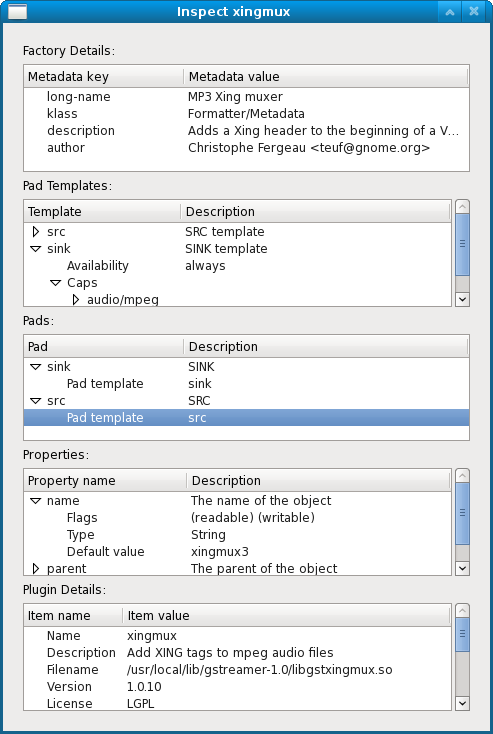
\includegraphics[width=110mm]{img/xingmux-factory-info-window.png}
  \caption{Okno informacyjne dla fabryki elementu \textit{xingmux}}
  \label{fig:xingmuxFactoryInfoWindow}
\end{figure}\paragraph{}\vspace{-3mm}
\textbf{Obszar roboczy programu} \\
Obszar roboczy jest głównym modułem programu. Służy do tworzenia modelu programu metodą \textit{Drag\&Drop}. Każdy element modelu programu jest reprezentowany w obszarze roboczym poprzez zielony bloczek (rysunek ~\ref{fig:sampleBlock}). Przy brzegach bloczka znajdują się piny, które odzwierciedlają gniazda oraz szablony gniazd w modelu programu. \\
Poniżej opisane zostały wszystkie funkcje, jakie oferuje obszar roboczy programu.
\begin{figure}[H]
  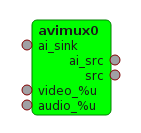
\includegraphics[width=35mm]{img/sample-block.png}
  \caption{Graficzna reprezentacja elementu \textit{avimux} w obszarze roboczym}
  \label{fig:sampleBlock}
\end{figure}
\begin{itemize}
  \setlength{\itemsep}{0em}

\item 
\textbf{Dodawanie elementów} - dodawanie elementów do modelu programu odbywa sie przy współpracy z inspektorem elementów. Aby dodać element, należy rozwinąć drzewo odpowiedniej wtyczki. Następnie, trzeba przeciągnąć dany element z inspektora elementów na obszar roboczy (rysunek ~\ref{fig:dragDropElement}). Po upuszczeniu obiektu, pojawia się okno z pytaniem o nazwę tworzonego elementu (rysunek ~\ref{fig:nameForElementWindow}).
\begin{figure}[H]
  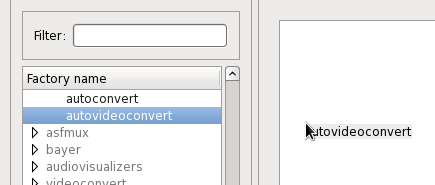
\includegraphics[width=0.95\textwidth]{img/drag-drop-element.png}
  \caption{Dodawanie elementów do obszaru roboczego metodą drag\&drop}
  \label{fig:dragDropElement}
\end{figure}
\item \textbf{Usuwanie elementów}\\ 
Aby usunąć element z modelu, należy kliknąć prawym przyciskiem myszy na danym elemencie.
\begin{figure}[H]
  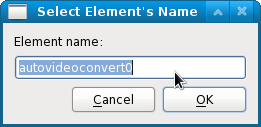
\includegraphics[width=0.6\textwidth]{img/name-for-element-window.png}
  \caption{Okno konfiguracji nazwy nowego elementu}
  \label{fig:nameForElementWindow}
\end{figure}

\item \textbf{Tworzenie połączeń} \\
W celu utworzenia połączenia, należy kliknąć lewym przyciskiem myszy na pin, który chcemy połączyć, a następnie trzeba przeciągnąć kursor na pin, z którym chcemy połączyć element źródłowy. Jeśl połączenie może być zrealizowane, podświetlone jest na zielono. W przypadku, gdy połączenie nie może być zrealizowane, połączenie podświetlone jest na kolor czerwony.
\item \textbf{Usuwanie połączeń} \\ 
Aby usunąć połączenie pomiędzy elementami, należy kliknąć prawym przyciskiem na danym połączeniu.
\item \textbf{Tworzenie gniazd na żądanie} \\
Szablony gniazd, które mogą być utworzone na żadanie, są wyświetlane w obszarze bloczka elementu jako piny. Aby utworzyć gniazdo na podstawie szablonu, wystarczy połączyć inny element z danym szablonem. Gniazdo zostanie utworzone automatycznie. Proces ten został zilustrowany na rysunku ~\ref{fig:onRequestPad}.
\begin{figure}[H]
  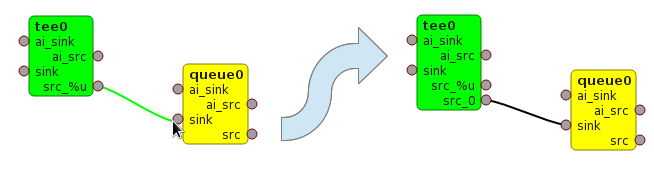
\includegraphics[width=14cm]{img/on-request-pad.png}
  \caption{Proces tworzenia gniazda na podstawie szablonu}
  \label{fig:onRequestPad}
\end{figure}
Po połączeniu pinu szablonu \textit{tee\_\%u} z gniazdem wejsciowym elementu \textit{qubbeue0}, zostało utworzone gniazdo \textit{src\_0}, które automatycznie zostało połączone z gniazdem \textit{sink}.
\begin{figure}[H]
  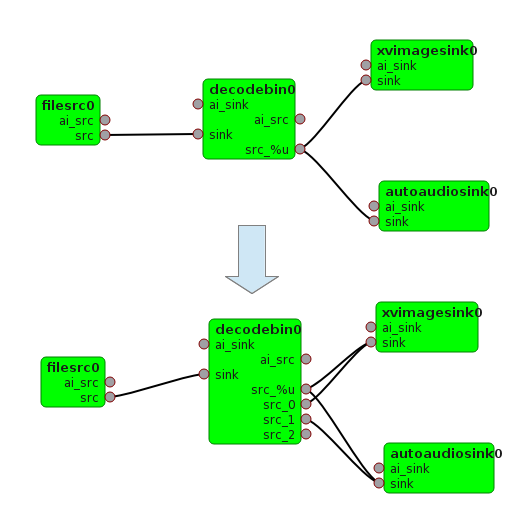
\includegraphics[width=14cm]{img/future-connections.png}
  \caption{Wykorzystanie połączeń przyszłościowych}
  \label{fig:futureConnections}
\end{figure}
\item \textbf{Tworzenie połączeń przyszłościowych} \\
Nie znając dokładnego formatu przychodzacych danych multimedialnych, użytkownik nie jest w stanie zaprojektować działającego modelu programu. Jednak często zdarza się, że podczas odtwarzania np. pliku multimedialnego, nie można przewidzieć, ile ścieżek jest w nim zawartych. \textit{Połączenia przyszłościowe} mają na celu rozwiązanie tego problemu. Korzystając z połączeń przyszłościowych, użytkownik może zaplanować połączenie pomiędzy dwoma elementami, które wystąpi tylko w przypadku, gdy dany strumień będzie dostępny.
Na rysunku ~\ref{fig:futureConnections} można zobaczyć przykładowe użycie połączeń przyszłościowych. Przed uruchomieniem programu, nie można określić, jakiego formatu dane pojawią się na wejściu elementu \textit{decodebin0}. Dlatego użytkownik może zaznaczyć, że w przypadku wystąpienia strumienia audio lub wideo, powinno wygenerować się połączenie pomiędzy dekoderem a jednym z rendererów. Można zauważyć, że dane multimedialne zawierały trzy strumienie (zostały wygenerowane trzy gniazda źródłowe w elemencie dekodującym). Użytkownik zaplanował jednak połączenia tylko dla dwóch gniazd, dlatego trzecie nie zostało podłaczone\\
\item \textbf{Tworzenie inteligentnych połączeń} \\
Każdy blok, zawierający piny wejściowe lub wyjściowe, posiada też tzw. \textit{inteligentne piny}, oznaczone w bloku jako \textit{ai\_sink} w przypadku pinów wejściowych, oraz \textit{ai\_src} w przypadku pinów wyjściowych. Kiedy użytkownik nie jest pewien tego, jakie gniazdo powinien wybrać dla danego połączenia, może skorzystać z \textit{inteligentnych połączeń}. Są to połączenia, w których występuje conajmniej jeden inteligentny pin. Po wykonaniu inteligentnego połączenia, zostanie ono zastapione przez najlepsze stałe połączenie. Proces inteligentnego łączenia przedstawia rysunek ~\ref{fig:aiConnectionProcess}. 
\begin{figure}[H]
  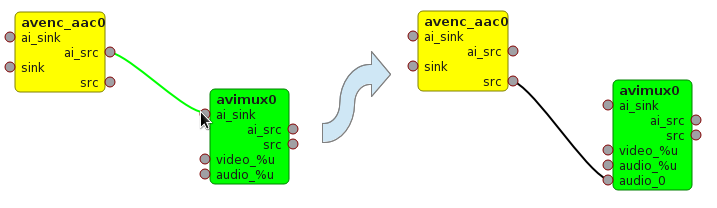
\includegraphics[width=150mm]{img/ai-connection-process.png}
  \caption{Proces inteligentnego łączenia pomiędzy audio enkoderem i elementem \textit{avimux0}}
  \label{fig:aiConnectionProcess}
\end{figure}
Po wykonaniu inteligentnego połączenia pomiędzy audio enkoderem \textit{avenc\_aac0} i elementu \textit{avimux0}, program wykonuje przeszukiwania, w celu wykonania najlepszego połączenia. Poprawnym wynikiem jest utworzenie połączenia pomiędzy gniazdem źródłowym enkodera i gniazdem wejściowym typu \textit{audio} elementu \textit{muxera}.
\end{itemize}\paragraph{}\vspace{-3mm}
\textbf{Wiersz poleceń} \\
Wiersz poleceń umożliwia budowę modelu na podstawie prostych komend interpretowanych przez program. Wiersz poleceń posiada również mechanizm podpowiadania składni (rysunek ~\ref{fig:commandLine}), który ma na celu przyśpieszenie i ułatwienie użytkownikowi pracy z programem. W przypadku słów kluczowych, wielkość liter nie ma znaczenia. Poniżej przedstawiona zostanie syntaktyka poszczególnych poleceń. 
\begin{figure}[H]
  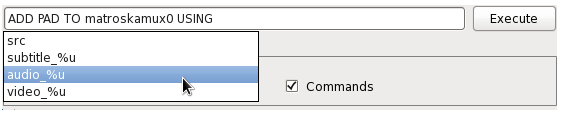
\includegraphics[width=140mm]{img/command-line.png}
  \caption{Mechanizm podpowiadania składni w wierszu poleceń}
  \label{fig:commandLine}
\end{figure}
\begin{itemize}
  \setlength{\itemsep}{0em}
\item \textbf{ADD} - dodaje element do modelu programu lub dodaje gniazdo do elementu.
\underline{Składnia:} \\
\texttt{ADD \\
\hspace*{2em} \{ELEMENT \textit{fabryka} [\textit{nazwa\_elementu}]\} | \\
\hspace*{2em} \{PAD TO \textit{element} USING \textit{szablon} [\textit{nazwa\_gniazda}]\} }
\begin{itemize}
\item \textit{fabryka} - nazwa fabryki, jaka ma zostać użyta do skonstruowania elementu.
\item \textit{nazwa\_elementu} - nazwa dla nowo utworzonego elementu (parametr opcjonalny).
\item \textit{element} - nazwa elementu, do którego dodane zostanie gniazdo.
\item \textit{szablon} - schemat, na podstawie którego zostanie utworzone gniazdo.
\item \textit{nazwa\_gniazda} - nazwa dla nowo utworzonego gniazda (parametr opcjonalny).
\end{itemize}
\underline{Przykłady:} \\
\texttt{ADD ELEMENT giosink} \\
\texttt{ADD ELEMENT fakesrc fake-generator} \\
\texttt{ADD PAD TO tee0 USING src\_\%u} \\
\texttt{ADD PAD to matroskamux0 USING subtitle\_\%u sub1}
\item \textbf{REMOVE} - usuwa element z modelu programu lub usuwa gniazdo z elementu. \\
\underline{Składnia:} \\
\texttt{REMOVE \\
\hspace*{2em} \{ELEMENT \textit{nazwa\_elementu}\} | \\
\hspace*{2em} \{PAD \textit{nazwa\_elementu}:\textit{nazwa\_gniazda}\}}
\begin{itemize}
\item \textit{nazwa\_elementu} - nazwa elementu, który ma zostać usunięty.
\item \textit{nazwa\_gniazda} - nazwa gniazda, które ma zostać usunięte.
\end{itemize}
\underline{Przykłady:} \\
\texttt{REMOVE ELEMENT videotestsrc0}
\texttt{REMOVE PAD matroskamux0:sub1}
\item \textbf{PROPERTY} - umożliwia zmianę właściwości elementu.
\underline{Składnia:} \\
\texttt{PROPERTY \textit{element} [\textit{właściwość} \textit{wartość}]}
\begin{itemize}
\item \textit{element} - nazwa elementu, którego właściwość będzie zmieniana.
\item \textit{właściwość} - nazwa właściwości, jaka powinna zostać zmieniona (parametr opcjonalny).
\item \textit{wartość} - nowa wartość dla zadanej właściwości (parametr opcjonalny). 
\end{itemize}
\underline{Przykłady:} \\
\texttt{PROPERTY videotestsrc0} \\
\texttt{PROPERTY filesink0 location /home/m.kolny/output.mkv} \\
\underline{Uwagi:} \\
Użycie polecenia \textit{PROPERTY} w wariancie jednoargumentowym nie spowoduje de facto zmiany żadnego parametru. Wynikiem wykonania takiego polecenia będzie za to wyświetlenia okna z listą wszystkich dostępnych parametrów dla danego elementu(rysunek ~\ref{fig:allPropertiesWindow}), z możliwością zmiany tych parametrów.
\begin{figure}[H]
  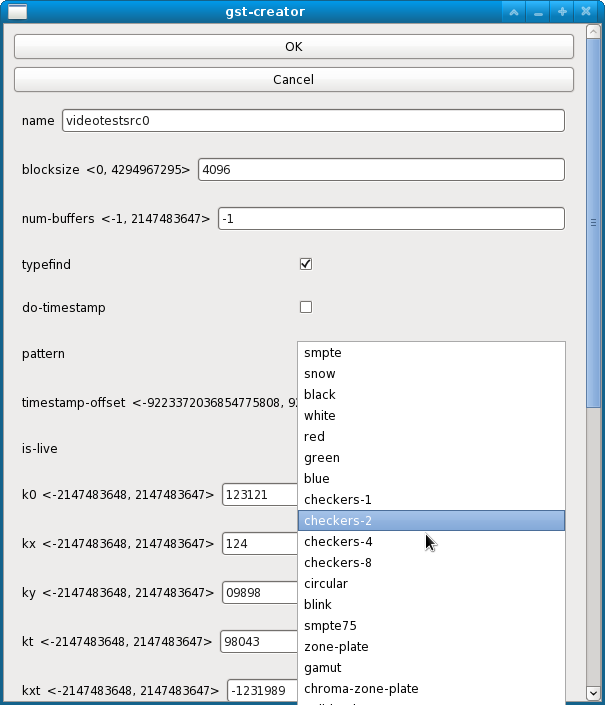
\includegraphics[width=150mm]{img/all-properties-window.png}
  \caption{Okno konfiguracji parametrów elementu \textit{videotestsrc0} - wynik wykonania polecenia \texttt{PROPERTY videoetstsrc0}}
  \label{fig:allPropertiesWindow}
\end{figure}
\item \textbf{STATE} - zmienia stan modelu programu. \\
\underline{Składnia:} \\
\texttt{STATE STOP | PAUSE | PLAY} \\
\underline{Przykłady:} \\
\texttt{STATE STOP} \\
\texttt{STATE PLAY}
\item \textbf{CONNECT} - łączy ze sobą elementy lub gniazda. \\
\underline{Składnia:} \\
\texttt{CONNECT \\
\hspace*{2em} \{ELEMENT \textit{element\_źródłowy} WITH \textit{element\_docelowy}\} \\
\hspace*{2em} | \\
\hspace*{2em} \{PAD \textit{element\_źródłowy}:\textit{gniazdo\_źródłowe} WITH \\
\hspace*{4em} \textit{element\_docelowy}:\textit{gniazdo\_docelowe}\} \\
\hspace*{2em} [FUTURE]}
\begin{itemize}
\item \textit{element\_źródłowy} - nazwa elementu źródłowego dla połączenia.
\item \textit{element\_docelowy} - nazwa elementu docelowego dla połączenia.
\item \textit{gniazdo\_źródłowe} - nazwa gniazda w elementcie źródłowym.
\item \textit{gniazdo\_docelowe} - nazwa gniazda w elementcie docelowym.
\end{itemize}
\underline{Przykłady:} \\
\texttt{CONNECT ELEMENT matroskademux0 WITH avdec\_aac0 FUTURE} \\
\texttt{CONNECT ELEMENT videotestsrc0 WITH xvimagesink0} \\
\texttt{CONNECT pad matroskademux0:video\_\%u WITH xvimagesink0:sink FUTURE}
\texttt{CONNECT ELEMENT audiotestsrc0:src WITH autoaudiosink0:sink} \\
\underline{Uwagi:} \\
Słowo kluczowe \texttt{FUTURE} powinno zostać użyte w przypadku, gdy dane gniazdo nie istnieje na etapie projektowania modelu programu, a jego istnienie jest zależne od formatu wejściowych danych multimedialnych.
\item \textbf{DISCONNECT} - rozłącza ze sobą elementy lub gniazda. \\
\underline{Składnia:} \\
\texttt{DISCONNECT \\
\hspace*{2em} \{ELEMENT \textit{element\_źródłowy} WITH \textit{element\_docelowy}\} \\
\hspace*{2em} | \\
\hspace*{2em} \{PAD \textit{element\_źródłowy}:\textit{gniazdo\_źródłowe} WITH \\
\hspace*{4em} \textit{element\_docelowy}:\textit{gniazdo\_docelowe}\}
}
\begin{itemize}
 \setlength{\itemsep}{0em}
\item \textit{element\_źródłowy} - element źródłowy istniejącego połączenia.
\item \textit{element\_źródłowy} - element docelowy istniejącego połączenia.
\item \textit{gniazdo\_źródłowe} - gniazdo źródłowe istniejącego połączenia.
\item \textit{gniazdo\_docelowe} - gniazdo docelowe istniejącego połączenia.
\end{itemize}
\underline{Przykłady:} \\
\texttt{DISCONNECT ELEMENT queue0 WITH xvimagesink0} \\
\texttt{DISCONNECT PAD videotestsrc0 WITH autovideosink0}
\end{itemize}\paragraph{}\vspace{-3mm}
\textbf{Konsola logowania zdarzeń programu} \\
Konsola umożlwia użytkownikowi śledzić listę komend, jakie skierował do programu. Pozwala również na podglądanie wiadomości pojawiających się na magistrali programu. Użytkownik ma możliwość wyboru źródeł pochodzenia informacji.
\paragraph{}\vspace{-3mm}
\textbf{Konsola logowania zdarzeń GStreamera} \\
Konsola wyświetla wszystkie wiadomości przydatne w procesie debugowania modelu programu, jakie pochodzą z biblioteki GStreamer. Użytkownik może wybrać, które z dostępnych informacji danego wpisu mają być wyświetlane. Dostępne są:
\begin{itemize}
 \setlength{\itemsep}{0em}
\item kategoria,
\item poziom ważności,
\item plik, z jakiego pochodzi dana wiadomość,
\item numer linii w pliku, z której wywołano funkcję wysyłającą wiadomość,
\item nazwa funkcji, z której została wysłana wiadomość,
\item treść wiadomości.
\end{itemize}
Ponadto użytkownik korzystając z przycisku \textit{Filter properties} ma możliwość ustawienia poziomu szczegółowości informacji debugujących. Okno konfiguracyjne (rysunek ~\ref{fig:debugLevelProperties}) pozwala użytkownikowi na ustawienie domyślnego poziomu szczegółowości, a także poziomu szczegółowości dla każdej z kategorii osobno. Po wybraniu domyślnego poziomu, i zatwierdzeniu wyboru przyciskiem \textit{OK}, wszystkie ustawienia dla konkretnych kategorii zostaną zapomniane, a poziom szczegółowości dla każdej kategorii zostanie ustawiony na wartość domyślnego poziomu.
\begin{figure}[H]
  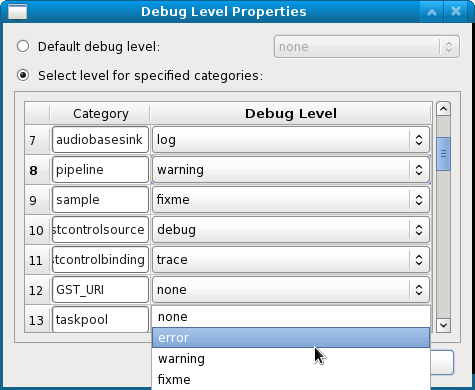
\includegraphics[width=130mm]{img/debug-level-properties.png}
  \caption{Okno konfiguracji zdarzeń biblioteki GStreamer}
  \label{fig:debugLevelProperties}
\end{figure}
Użytkownik ma możliwość wyboru jednego z ośmiu poziomów logowania:
\begin{enumerate}
 \setlength{\itemsep}{0em}
\item brak logowania (\textit{none}),
\item logowanie błędów (\textit{error}),
\item logowanie ostrzeżeń (\textit{warning}),
\item logowanie braków w implementacji biblioteki (\textit{fixme}),
\item logowanie informacji na temat ogólnego przebiegu działania programu (\textit{info}),
\item logowanie informacji na temat rzadko występujących lub nieoczekiwanych zdarzeń (\textit{info}),
\item logowanie informacji które mogą być przydatne dla użytkownika, ale są bardzo oczywiste (\textit{log}),
\item dokładne śledzenie przebiegu wykonania programu (\textit{trace}).
\end{enumerate}
Poziomy logowania mają strukturę hierarchiczną - włączając poziom logowania \textit{info}, zostaje automatycznie włączony poziom logowania \textit{fixme}, \textit{warnings} oraz \textit{error}.
\subsubsection{Kreator wtyczek}
Biblioteka GStreamer udostępnia użytkownikowi interfejs do pisania wtyczek. Przygotowanie szablonu do napisania własnej wtyczki jest jednak bardzo czasochłonne. Kreator wtyczek ma na celu przyspieszenie procesu tworzenia nowych wtyczek, poprzez wygenerowanie szablonu, zawierającego podstawowe informacje, oraz prostą implementację podstawowych funkcjonalności.
\begin{figure}[H]
  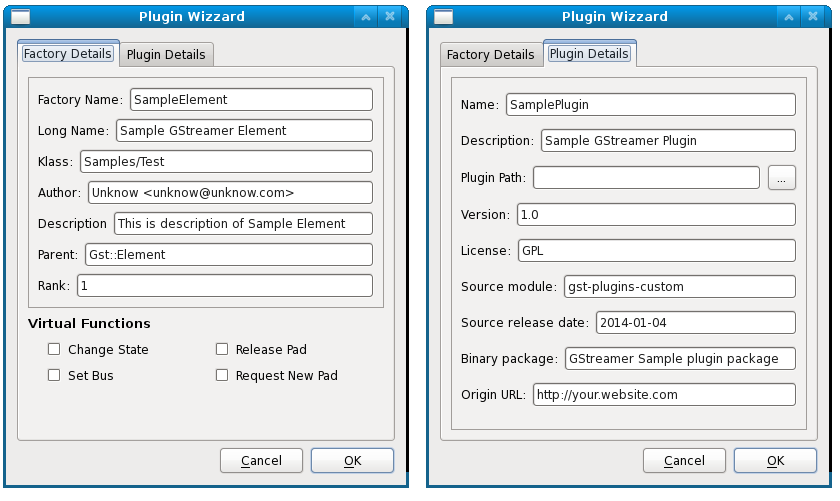
\includegraphics[width=160mm]{img/plugin-wizzard.png}
  \caption{Karty kreatora wtyczek}
  \label{fig:pluginWizzard}
\end{figure}
Kreator pozwala również na utworzenie fabryki elementów. W kolejnych wersjach programu funkcjonalność ta zostanie rozbudowana o możliwość wygenerowania większej ilości fabryk w ramach jednej wtyczki.
Okno kreatora podzielone jest na dwie zakładki (rysunek ~\ref{fig:pluginWizzard}). Pierwsza dotyczy informacji na temat fabryki zawartej we wtyczce, druga natomiast pozwala na zdefiniowanie szczegółów wtyczki.

\noindent
Oprócz metadanych fabryki elementów, użytkownik może również zażądać wygenerowania niektórych funkcji wirtualnych:
\begin{itemize}
  \setlength{\itemsep}{0em}
\item zmiany stanu,
\item zwolnienia gniazda,
\item ustawienia magistrali,
\item żądania nowego gniazda.
\end{itemize}
\subsubsection{Generator kodu}
Przydatnym dla programisty narzędziem może okazać się generator kodu. Model programu, który został stworzony przez użytkownika, jest przekładany na kod źródłowy, i jest zapisywany do pliku. Okno generatora przedstawiono na rysunku ~\ref{fig:codeGenerator}. Wymagane jest jedynie podanie ścieżki do wygenerowanego pliku, oraz wybranie języka wygenerowanego kodu źródłowego.
\begin{figure}[H]
  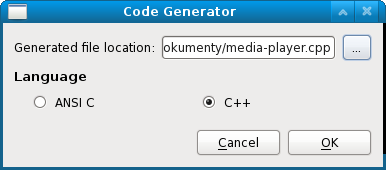
\includegraphics[width=80mm]{img/code-generator.png}
  \caption{Okno generatora kodu}
  \label{fig:codeGenerator}
\end{figure}
Aktualnie program generuje tylko kod źródłowy w języku C++ w oparciu o wrapper gstreamermm, natomiast następna wersja oprogramowania przewiduje również możliwość generowania kodu w języku ANSI C, korzystając z bezpośrednich wywołań funkcji bibliotecznych.\\
Publiczny interfejs wygenerowanej klasy, gotowej do użycia we własnym programie, przedstawiony jest na listingu ~\ref{codeGeneratorPublicApi}.
\begin{lstlisting}[caption=Publiczny interfejs klasy stworzonej przez generator kodu, label=codeGeneratorPublicApi]
class Creator
{
public:
	virtual ~Creator(){}

	Glib::RefPtr<Gst::Pipeline> get_pipeline();
}
\end{lstlisting}
Metoda \texttt{get\_pipeline()} zwraca strumień przetwarzający dane multimedialne.\\
Wraz z wygenerowanym kodem, dołączane jest również przykładowe użycie klasy.\\
Kod źródłowy wygenerowany przez generator jest zgodny ze standardem języka C++11.
\cleardoublepage
\section{Specyfikacja wewnętrzna}
\subsection{Rozwój biblioteki gstreamermm}
Biblioteka gstreamermm miała swój początek na początku 2008 roku. Wydanie dotyczyło wersji 0.9.1 biblioteki GStreamer, dlatego biblioteka-adapter otrzymała również taki numer. Biblioteka była rozwijana przez dwóch programistów: José Alburquerque oraz Murraya Cumminga. Jednak po wydaniu wersji 0.10.11, projekt nie był dalej rozwijany. Ponieważ wykorzystuję bibliotekę GStreamer, postanowiłem kontynuować projekt gstreamermm.
\subsubsection{Zmiany w blibliotece GStreamer}
Nowa wersja (1.0) biblioteki GStreamer wnosiła wiele zmian w stosunku do poprzedniej wersji biblioteki (0.10), adapter więc wymagał też wielu poprawek. 
\begin{itemize}
 \setlength{\itemsep}{0em}
  \item Wielu zmian dokonano w klasie \textit{GstBuffer}, która reprezentuje bufor danych w bibliotece GStreamer. Główna zmiana polegała na wprowadzeniu innego sposobu organizacji pamięci w buforze.
  \item Wiele funkcji związanych z gniazdami, zostało opartych o zapytania.
  \item Usunięte zostały wszystkie funkcje, oznaczone jako przestarzałe (ang. \textit{deprecated}).
\end{itemize}
Ponadto, w nowej wersji biblioteki GStreamer niektóre nazwy funkcji zostały zastąpione bardziej obrazowymi odpowiednikami. Zmieniała się również lista argumentów kilku funkcji.
Wszystkie powyższe zmiany musiały zostać uwzględnione w bibliotece adaptera.
\subsubsection{Wdrożenie nowego systemu testowania}
Do wersji 0.10, biblioteka gstreamermm nie była wyposażona w zautomatyzowany system testowania kodu. Tworzone były proste programy testujące, które należało uruchamiać ręcznie, a następnie śledzić wyniki wyświetlane na konsoli. Było to niewygodne, zwłaszcza dla dużej ilości testów. W wersji 1.0 biblioteki gstreamermm postanowiłem użyć popularnego systemu do testów automatycznych, \textbf{Google Test}. Po przeniesieniu testów na wspomniany wcześniej system, mogłem o wiele częściej uruchamiać wszystkie testy, i w łatwy sposób analizować rezultaty ich wykonania (rysunek ~\ref{fig:gtestScreen}). Użycie platformy testującej pozwoliło mi również na łatwiejsze pisanie testów.
\begin{figure}[H]
  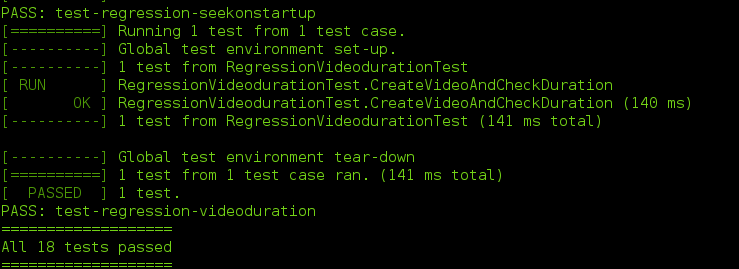
\includegraphics[width=150mm]{img/gtest-screen.png}
  \caption{Fragment zrzutu ekranu uruchomionego systemu Google Test dla projektu gstreamermm}
  \label{fig:gtestScreen}
\end{figure}
\subsubsection{Adaptacja modułu pisania wtyczek}
Biblioteka GStreamer opiera się o wtyczki, umożliwiające wprowadzenie do systemu dowolnego algorytmu. Adapter gstreamermm w wersji wcześniejszej, niż 1.0, nie posiadał oficjalnie wsparcia do pisania własnych wtyczek w języku C++. Powstała jednak nieoficjalna implementacja\cite{pepergithub}, która oferowała programiście wsparcie dla pisania własnych wtyczek. Zaaplikowałem moduł do oficjalnego repozytorium. Dopisałem również brakującą klasę, która ułatwiała programiście dostęp do klasy danego elementu wtyczki.
\subsubsection{Poprawki w generatorach kodu}
Przy rozwijaniu projektu gstreamermm, wystąpiło kilka problemów, które należało rozwiązać po stronie generatora kodu. Jednym z nich był brak możliwości wprowadzenia wartości typu wyliczeniowego jako definicji wieloargumentowej. Na listingu ~\ref{badEnumForGenerator} pokazany został kod, który z punktu widzenia generatora kodu, był niepoprawny.
    \begin{lstlisting}[caption=Przykładowy fragment niepoprawnego z punktu widzenia generatora kodu źródłowego, label=badEnumForGenerator]
typedef enum {
  GST_QUERY_UNKNOWN      = GST_QUERY_MAKE_TYPE
(0, 0),
  GST_QUERY_POSITION     = GST_QUERY_MAKE_TYPE 
(10, FLAG(BOTH)),
  GST_QUERY_DURATION     = GST_QUERY_MAKE_TYPE 
(20, FLAG(BOTH)),
    \end{lstlisting}

Po wygenerowaniu kodu na podstawie powyższej definicji, oczekiwanym wynikiem jest fragment przedstawiony na listingu ~\ref{expectedGeneratedEnum}, natomiast generator tworzył kod, zaprezentowany na listingu ~\ref{outputGeneratedEnum}. Poprawienie błędu polegało na zmodyfikowaniu reguł dla wyrażeń regularnych generatora.

    \begin{lstlisting}[caption=Oczekiwany wynik działania generatora kodu, label=expectedGeneratedEnum]
(define-flags-extended QueryType
  (in-module "Gst")
  (c-name "GstQueryType")
  (values
    '("unknown" "GST_QUERY_UNKNOWN" 
"GST_QUERY_MAKE_TYPE (0,  0)")
    '("position" "GST_QUERY_POSITION" 
"GST_QUERY_MAKE_TYPE (10,  FLAG(BOTH))")
    '("duration" "GST_QUERY_DURATION" 
"GST_QUERY_MAKE_TYPE (20,  FLAG(BOTH))")
    \end{lstlisting}

    \begin{lstlisting}[caption=Błędnie wygenerowany kod przez generator, label=outputGeneratedEnum]
(define-enum-extended QueryType
  (in-module "Gst")
  (c-name "GstQueryType")
  (values
    '("gst-query-unknown" "GST_QUERY_UNKNOWN" 
"GST_QUERY_MAKE_TYPE (0")
    '("0)" "0)" "(GST_QUERY_MAKE_TYPE (0) + 1")
    '("gst-query-position" "GST_QUERY_POSITION" 
"GST_QUERY_MAKE_TYPE (10")
    '("flag(both))" "FLAG(BOTH))" 
"(GST_QUERY_MAKE_TYPE (10) + 1")
    '("gst-query-duration" "GST_QUERY_DURATION" 
"GST_QUERY_MAKE_TYPE (20")
    '("flag(both))" "FLAG(BOTH))" 
"(GST_QUERY_MAKE_TYPE (20) + 1")
    \end{lstlisting}

\subsection{Struktura programu gst-creator}
Struktura programu podzielona jest na biblioteki, które gromadzą w sobie powiązane logicznie klasy. Poniżej przedstawione zostały wszystkie moduły, wraz z opisem oraz listą klas.
\subsubsection{Moduł Commands}
Biblioteka zawiera klasy implementujące wzorzec projektowy \textit{Commands}. Obiekty tych klas wykorzystywane są do operacji na modelu programu.
\paragraph{}
\textbf{Lista klas}
\vspace{-2mm}
\begin{itemize}
 \setlength{\itemsep}{0em}
\item \texttt{CommandListener} - definiuje interfejs, jaki musi spełniać obiekt nasłuchujący wykonania komend. Wszystkie metody w klasie mają swoją własną implementację, dla tego obiekt nasłuchujący może implementować tylko wybrane metody nasłuchujące zdarzenia.
\item \texttt{Command} - klasa bazowa dla wszystkich klas będących komendami w bibliotece. Posiada abstrakcyjną metodę \texttt{run\_command(std::vector<CommandListener*> listeners)}, która musi być zdefiniowana w klasie reprezentującej konkretną komendę. Metoda odpowiedzialna jest za uruchomienie zdefiniowanego wcześniej polecenia. Oprócz tego klasa definiuje pole prywatne przechowujące typ komendy.
\item \texttt{AddCommand} - komenda odpowiedzialna za dodawanie elementów do modelu programu lub gniazd do istniejących elementów. Definiuje metodę statyczną \\
\texttt{static AddCommand* from\_args(const std::vector<std::string>\& args, const Glib::RefPtr<Gst::Pipeline>\& model);}\\
która odpowiedziana jest za wygenerowanie obiektu komendy na podstawie listy argumentów.
W ramach klasy została również zdefiniowana metoda \\
\texttt{static std::vector<std::string> get\_suggestions(const std::vector<std::string>\& args, const Glib::RefPtr<Gst::Pipeline>\& model);}\\
odpowiedzialna za zwrócenie podpowiedzi następnego argumentu, na podstawie już istniejącej listy argumentów.\\
Metody \texttt{from\_args} oraz \texttt{get\_suggestion} zdefiniowane są również w pozostałych klasach komend.
\item \texttt{ConnectCommand} - komenda łącząca ze soba gniazda. Uruchomienie komendy może skutkować wywołaniem komendy \texttt{AddCommand} tworzącą gniazdo. Taka sytuacja może wystąpić w przypadku tworzenia inteligentnego połączenia.
\item \texttt{DisconnectCommand} - komenda usuwająca połączenia pomiędzy elementami.
\item \texttt{PropertyCommand} - komenda zmieniająca właściwość elementu. W szczególnym przypadku może też posłużyć jako komenda wywołująca okno konfiguracji właściwości.
\item \texttt{RemoveCommand} - komenda usuwająca elementy lub gniazda.
\item \texttt{StateCommand} - komenda zmiany stanu modelu programu.
\end{itemize}
\subsubsection{Moduł Console}
Moduł odpowiada za wiersz poleceń. Zawiera klasy odpowiadające za logike oraz za widok konsoli. 
\cleardoublepage
\paragraph{}
\textbf{Lista klas}
\vspace{-2mm}
\begin{itemize}
  \setlength{\itemsep}{0em}
\item \texttt{CommandParser} - klasa parsera komend. Na podstawie tekstu wprowadzonego przez użytkownika, parser generuje instancję klasy \texttt{Command}. Następnie komenda jest zwracana programiście, i może być uruchomiona w dowolnej chwili.
\item \texttt{ConsoleView} - klasa widoku konsoli. Realizuje operacje związane z interfejsem użytkownika - wyświetla podpowiedzi, uruchamia parser komend, daje użytkownikowi możliwość wykonania poleceń.
\end{itemize}
\subsubsection{Moduł controller}
Biblioteka ta dostarcza zestaw klas realizujących podstawową logikę głównego okna programu oraz dodatkowych narzędzi (generatora kodu oraz kreatora wtyczek). 
\paragraph{}
\textbf{Lista klas}
\vspace{-2mm}
\begin{itemize}
  \setlength{\itemsep}{0em}
\item \texttt{CodeGenerator} - klasa generująca kod źródłowy na podstawie modelu programu.
\item \texttt{FileLoader} - klasa odpowiedzialna za załadowanie pliku projektu do programu.
\item \texttt{FileWriter} - klasa realizuje funkcjonalność zapisuj stworzonego przez użytkownika projektu do pliku.
\item \texttt{MainController} - klasa głównego kontrolera, odpowiedzialna jest głównie za wykrywanie zmian zachodzących w modelu programu.
\item \texttt{FactoryInfo} - przechowuje informacje na temat fabryki elementów, jaka ma zostać wygenerowana przez kreator wtyczek. Generuje również kod źródłowy klasy fabryki.
\item \texttt{PluginInfo} - klasa przechowująca informacje na temat wtyczki dla kreatora wtyczek. Ponadto generuje kod źródłowy klasy wtyczki.
\item \texttt{PluginCodeGenerator} - główna klasa kreatora wtyczek. Uruchamia generator kodu źródłowego dla fabryki oraz wtyczki, zapisuje kod do pliku.
\end{itemize}
\subsubsection{Moduł FactoryInspector}
Moduł FactoryInspector udostępnia programiście klasy umożliwiające wyświetlanie informacji na temat danej fabryki elementów biblioteki GStreamer. 
\paragraph{}
\textbf{Lista klas}
\vspace{-2mm}
\begin{itemize}
  \setlength{\itemsep}{0em}
\item \texttt{FactoryInspectorView} - klasa odpowiada za prezentację wszystkich dostępnych informacji o fabryce elementów. 
\item \texttt{PropertyInspectorView} - klasa przedstawia listę właściwości dostępnych w ramach danej fabryki. Jest wykorzystywana w konstrukcji obiektu klasy \texttt{FactoryInspectorView}.
\item \texttt{VariousPropertyInspectorView} - klasa wykorzystywana jest do wyświetlania informacji na temat właściwości elementu o następujących typach:
  \begin{itemize}
    \setlength{\itemsep}{0em}
  \item \texttt{GParamSpecEnum},
  \item \texttt{GParamSpecFlags},
  \item \texttt{GParamSpecObject},
  \item \texttt{GParamSpecBoxed},
  \item \texttt{GParamSpecPointer},
  \item \texttt{GArray},
  \item \texttt{GstParamSpecFraction}.
  \end{itemize}
\end{itemize}
Powyższe typy są niestandardowe pod względem wyświetlania ich w interfejsie użytkownika, dla tego ich obsługa nie została zaimplementowana w klasie \texttt{PropertyInspectorView}.
\subsubsection{Moduł gui}
Biblioteka gui gromadzi w sobie klasy, jakie używane są do tworzenia okien programu. Wygląd okna określany jest poprzez plik \textit{ui}, będące plikiem opisu graficznego interfejsu. Na jego podstawie generowany jest kod klasy widoku. 
\paragraph{}
\textbf{Lista klas}
\vspace{-2mm}
\begin{itemize}
  \setlength{\itemsep}{0em}
\item \texttt{CodeGeneratorDialog} - okno dialogowe dla generatora kodu źródłowego.
\item \texttt{MainWindow} - główne okno programu.
\item \texttt{PluginWizardDialog} - okno dialogowe dla kreatora wtyczek.
\end{itemize}
\subsubsection{Moduł Logger}
Zadaniem biblioteki Logger jest dostarczenie zestawu klas umożliwiających prezentowanie użytkownikowi informacji wychodzących z aplikacji. 
\paragraph{}
\textbf{Lista klas}
\vspace{-2mm}
\begin{itemize}
  \setlength{\itemsep}{0em}
\item \texttt{GstLogger} - klasa odpowiedzialna za prezentacje wiadomości pochodzących z biblioteki GStreamer przydatnych do debugowania programu. Dziedziczy po klasie \texttt{QWidget} i jest używana jako oddzielny komponent graficznego interfejsu użytkownika.
\item \texttt{GstLoggerProperties} - wykorzystywana jest do określania, jakie wiadomości mają być wysyłane z biblioteki GStreamer, i jakie mają zostać wyświetlane w klasie \texttt{GstLogger}.
\item \texttt{LoggerView} - klasa odpowiada za przechwytywanie i wyświetlanie wiadomości z magistrali strumienia GStreamer, a także innych komunikatów aplikacji. Klasa umożliwia filtrowanie wiadomości na podstawie źródła pochodzenia wiadomości.
\end{itemize}
\subsubsection{Moduł ObjectInspector}
Biblioteka odpowiada za funkcjonalność inspektora elementów. Implementuje klasy związane z wyświetlaniem dostępnych wtyczek i fabryk.
\paragraph{}
\textbf{Lista klas}
\vspace{-2mm}
\begin{itemize}
  \setlength{\itemsep}{0em}
\item \texttt{ObjectInspectorFilter} - klasa pomocnicza, wykorzystywana w wyszukiwarce wtyczek i fabryk. Jest odpowiedzialna za filtrowanie wyników na podstawie wpisanego przez użytkownika tekstu.
\item \texttt{ObjectInspectorItem} - klasa obiektu pojedynczego wpisu w inspektorze elementów. 
\item \texttt{ObjectInspectorModel} - klasa-model inspektora elementów. Ładuje listę wtyczek i fabryk na podstawie informacji zawartych w bibliotece.
\item \texttt{ObjectInspectorView} - klasa widoku inspektora elementów. Implementuję metodę przeciągania elementu z inspektora elementów. Element ten jest następnie wykorzystywany w obszarze roboczym.
\item \texttt{PluginItem} - klasa pochodna klasy ObjectInspectorItem. Reprezentuje element wtyczki.
\end{itemize}  
\subsubsection{Moduł Properties}
W bibliotece glibmm, na której bazuje biblioteka gstreamermm, brakuje klas, które bardzo dobrze odzwierciedlałyby właściwości typów używanych w bibliotece GStreamer. Biblioteka Properties jest uzupełnieniem tego braku. Rozszerza też podstawową funkcjonalność właściwości o dołączenie dla  danego typu graficznego elementu pozwalającego na zmianę wartości. 
\paragraph{}
\textbf{Lista klas}
\vspace{-2mm}
\begin{itemize}
  \setlength{\itemsep}{0em}
\item \texttt{Property} - klasa bazowa dla pozostałych klas reprezentujących właściwość danego typu. Definiuje również metodę budującą obiekt  klas właściwości konkretnego typu, na podstawie opisu właściwości.
\item \texttt{PropertyBoolean} - klasa właściwości typu \texttt{boolean}.
\item \texttt{PropertyCaps} - klasa właściwości typu \texttt{Gst::Caps}.
\item \texttt{PropertyEnum} - klasa właściwości typu wyliczeniowego.
\item \texttt{PropertyNumeric} - klasa właściwości typu numerycznego. Jest to klasa szablonowa, ze konkretyzacjami dla typów \texttt{double}, \texttt{float}, \texttt{int}, \texttt{unsigned int}, \texttt{gint64}, \texttt{guint64}, \texttt{long} oraz \texttt{unsigned long}.
\item \texttt{PropertyString} - klasa właściwości typu \texttt{char*}.
\item \texttt{PropertyWidget} - komponent graficzny, który agreguje w sobie wszystkie komponenty właściwości danego elementu biblioteki GStreamer. Posiada metodę zapisu zmienionych parametrów.
\end{itemize}
\subsubsection{Moduł qnelibrary}
Biblioteka qnelibrary\cite{algoholic} służy do konstruowania schematów blokowych. Biblioteka posiada bardzo proste API. Dzięki licencji, na jakiej wypuszczone zostało to oprogramowanie (BSD), mogłem w swobodny sposób modyfikować poszczególne klasy biblioteki, i dostosowywać je do swoich potrzeb.
\paragraph{}
\textbf{Lista klas}
\vspace{-2mm}
\begin{itemize}
 \setlength{\itemsep}{0em}
\item \texttt{QNEBlock} - klasa pojedynczego bloczka. Agreguje w sobie piny, jest graficzną reprezentacją elementu w GStreamer. Dla własnego użytku zaimplementowałem metodę sprawdzającą, czy dany blok zawiera port z podanym modelem (metoda \texttt{find\_port}).
\item \texttt{QNEPort} - reprezentuje pojedynczy pin w bloku, jest odzwierciedleniem gniazda w elemencie biblioteki GStreamer. Abym mógł użyć te klasy w swoim projekcie, musiałem zaimplementować min. metody umożliwiające ustawienie modelu dla danego pinu czy metodę sprawdzającą, czy dany port może być podłączony do innego portu (pierwotnie biblioteka zakłada, że każdy port wyjściowy może być łączony z portem wejściowym za wyjątkiem portów w ramach jednego bloku, więc zaawansowane sprawdzanie nie było potrzebne).
\item \texttt{QNEConnection} - klasa odzwierciedla połączenie w bibliotece GStreamer. Połączenie wg założeń miało być jednokolorowe (domyślnie czarne). Konieczne było dopisanie funkcjonalności umożliwiającej zmianę koloru połączenia, w zależności od jego stanu (metoda \texttt{connectColor}).
\end{itemize}
\subsubsection{Moduł utils}
Biblioteka utils gromadzi w sobie zestaw narzędzi w postaci statycznych metod, których chciałem użyć w różnych miejscach programu, a których brakuje w bibliotece GStreamer czy języku C++.
\paragraph{}
\textbf{Lista klas}
\vspace{-2mm}
\begin{itemize}
 \setlength{\itemsep}{0em}
\item \texttt{EnumUtils} - jest to klasa generowana automatycznie, na podstawie pliku \textit{Command.h} w module \textit{Commands}. Generator kodu został napisany w języku Perl (plik \textit{enum\_string\_generator.pl}, i jest wywoływany przy każdej kompilacji programu.
Zadaniem klasy jest dostarczenie metod operujących na typach wyliczeniowych. Klasa pozwala na konwersję pomiędzy wartościami typu wyliczeniowego i typu łańcucha znaków (metody \texttt{enum\_to\_string}, \texttt{string\_to\_enum}), czy pobranie wszystkich zdefiniowanych wartości typu wyliczeniowego w postaci wektora łańcuchów znaków (metoda \texttt{get\_string\_values}).
\item \texttt{GstUtils} - klasa definiuje metody pomocnicze, jakich zabrakło mi w bibliotece GStreamer. Zdefiniowane są tam metody przeszukujące elementy, czy metody realizujące bardziej zaawansowane sprawdzanie możliwości połączenia pomiędzy elementami.
\item \texttt{Linkage} - prosta struktura reprezentująca pojedyncze połączenie.
\item \texttt{StringUtils} - jest to zbiór metod ułatwiających pracę z łańcuchami znaków.
\end{itemize}
\subsubsection{Moduł Workspace}
Biblioteka Workspace odpowiada za poprawne działanie obszaru roboczego, na którym odbywa się graficzne projektowanie modelu programu. Jest ściśle powiązana z biblioteką qnelibrary.
\paragraph{}
\textbf{Lista klas}
\vspace{-2mm}
\begin{itemize}
  \setlength{\itemsep}{0em}
\item \texttt{WorkspaceWidget} - klasa pochodna klasy \texttt{QWidget}, przedstawia kontrolkę obszaru roboczego. Ponadto klasa implementuje fragment interfejsu \texttt{CommandListener}, dzięki czemu zmiany w modelu programu są od razu widoczne w graficznej reprezentacji projektu. \\
Klasa implementuje wszystkie funkcje, jakie potrzebne są podczas projektowania graficznego (przesuwanie blokczków, łączenie pinów, usuwanie połączeń, elementów).
\end{itemize}
\cleardoublepage
\section{Testowanie oprogramowania}
Oprogramowanie gst-creator przeszło szereg testów, które dowiodły poprawności programu.\\
Główne testy składały się z jedenastu etapów:
\begin{enumerate}
  \setlength{\itemsep}{0em}
\item Utworzenie modelu programu.
\item Kilkukrotna zmiana stanu modelu programu.
\item Wprowadzenie modelu programu w stan zatrzymania.
\item Zapis projektu.
\begin{figure}[H]
  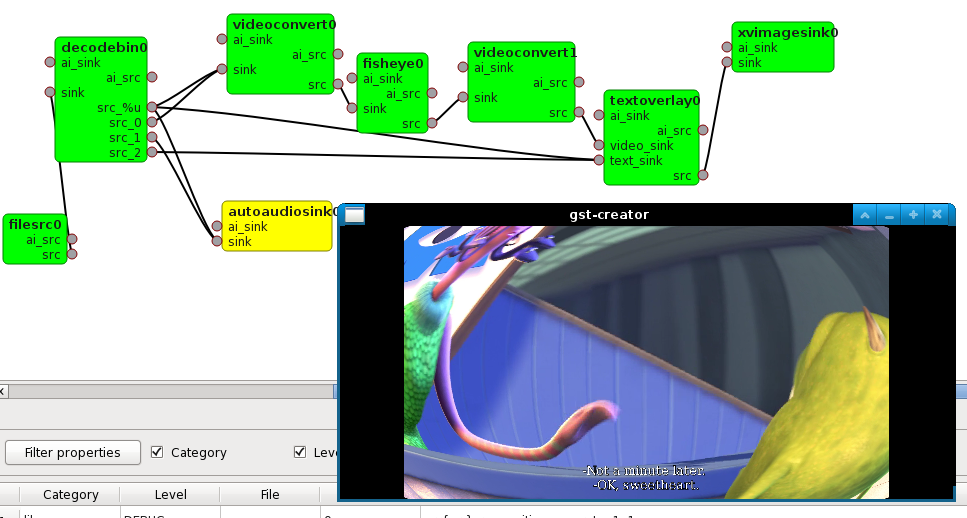
\includegraphics[width=160mm]{img/main-test-screen1.png}
  \caption{Odtwarzacz multimedialny stworzony w aplikacji gst-creator, z zastosowaniem filtra \textit{fisheye}. Fragment filmu \textit{Monsters} \cite{monstersDownloadPage}}
  \label{fig:mainTestScreen1}
\end{figure}
\item Załadowanie projektu. 
\item Kilkukrotna zmiana stanu modelu programu.
\item Zamknięcie aplikacji.
\item Uruchomenie aplikacji.
\item Kilkukrotna zmiana stanu modelu programu.
\item Wygenerowanie kodu źródłowego na podstawie modelu programu.
\item Kompilacja źródeł i uruchomienie aplikacji.
\end{enumerate}
Rysunki ~\ref{fig:mainTestScreen1} oraz ~\ref{fig:mainTestScreen2} przedstawiają przykładowe programy stworzone za pomocą aplikacji gst-creator, które wykorzystywane były w testach.
\begin{figure}[H]
  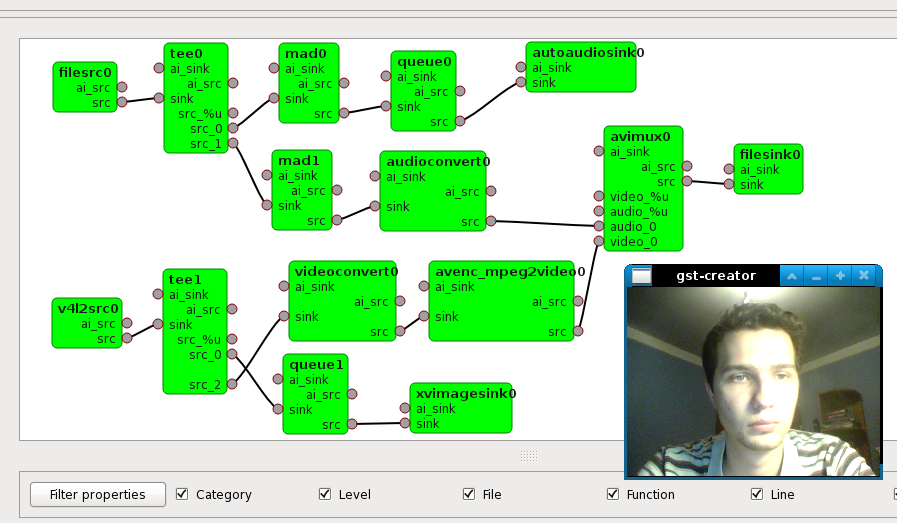
\includegraphics[width=160mm]{img/main-test-screen2.png}
  \caption{Program odtwarzający plik audio oraz obraz z kamery, jednocześnie zapisując obydwa strumienie do pliku}
  \label{fig:mainTestScreen2}
\end{figure}


\subsection{Testy pojedynczych modułów}
Wykonałem również testy pojedynczych modułów programu.
\begin{itemize}
  \setlength{\itemsep}{0em}
\item Moduł konsoli testowany był poprzez wprowadzanie (często niepoprawnych) poleceń, i sprawdzanie reakcji programu na te polecenia.
\item Kreator wtyczek został sprawdzony poprzez wygenerowanie kilkunastu wtyczek z różnymi parametrami. Wygenerowany kod był następnie kompilowany, a wtyczka sprawdzana została programem \textbf{gst-inspect} wchodzącym w skład pakietu GStreamer.
\item Mechanizm zmiany właściwości przetestowałem wprowadzając poprawne oraz niepoprawne wartości dla każdego z dostępnych typów. Sprawdzałem, czy program odpowiednio zapisze poprawne wartości, oraz czy zachowa się w sposób oczekiwany przy niepoprawnych wartościach.
\item Moduł wyświetlania informacji o wtyczkach i fabrykach obiektów testowany był za każdym razem, gdy szukałem informacji na temat danego obiektu.
\end{itemize}
\cleardoublepage
\section{Wnioski}
W ramach projektu udało mi się zrealizować wszystkie założenia projektowe. Korzystając z oprogramowania, użytkownik może w swobodny sposób tworzyć programy przetwarzające strumienie multimedialne, które później może zastąpić kodem źródłowym, i użyć w swoim własnym programie. 

Zaimplementowany został również mechanizm zapisu projektu do pliku, dzięki czemu użytkownik w każdej chwili będzie mógł zmodyfikować swój projekt. 

Stworzony został moduł pozwalający na śledzenie wiadomości pochodzących z biblioteki GStreamer z możliwością filtrowania poziomu ważności informacji oraz ich pochodzenia.

Dodatkowo, w programie zaimplementowano funkcje, które nie były przewidziane w założeniach projektowych, ale mogą przydać się użytkownikowi podczas pracy z programem. Pierwsza z funkcji, to narzędzie kreatora wtyczek, dzięki któremu w łatwy sposób można wygenerować szablon dla własnej wtyczki. 

Drugą istotną funkcją jest wiersz poleceń, dzięki któremu użytkownik może budować model programu używając tylko i wyłącznie klawiatury.

Oprócz tego, w programie zawarłem też funkcjonalność przeglądania informacji na temat dostępnych wtyczek oraz fabryk elementów, co również jest bardzo przydatne na etapie prototypowania aplikacji.
\cleardoublepage
\begin{thebibliography}{9}

\bibitem{gstmainpage}
  http://gstreamer.freedesktop.org [9.12.2013]
\bibitem{devgnomepage}
  https://developer.gnome.org [9.12.2013]
\bibitem{pepergithub}
  https://github.com/peper0/gstreamermm-plugins [10.12.2013]
\bibitem{algoholic}
  http://algoholic.eu [28.12.2013]
\bibitem{monstersDownloadPage}
  http://www.auby.no/files/video\_tests/ [31.12.2013]
\bibitem{qtDoc}
  http://qt-project.org/doc/qt-5.0/qtdoc/index.html [31.12.2013]
\bibitem{alex1}
  Andrei Alexandrescu , \textit{Nowoczesne projektowanie w C++. Uogólnione implementacje wzorców projektowych}, Wyd. 1, Gliwice, HELION, 2011, ISBN 978-83-246-3301-2.
\bibitem{meyers1}
  Scott Meyers , \textit{Język C++ bardziej efektywny}, Wydawnictwa Naukowo Techniczne, 1998, ISBN 83-204-2307-4.
\end{thebibliography}
\end{document}
